\section{Method}
\label{sec:method}

\subsection{Q/K Address Construction}
\label{sec:qk_address}

We target QKFormer attention modules and hook their binary Q/K spikes and
token/channel gating signals. Crucially, we do \emph{not} use an entire
$d$-dimensional Q/K vector as one $2^{2d}$ address. Each scalar module response
is indexed by a compact local state. For Token-QK attention, the address is
\begin{equation}
 a^{\mathrm{TQK}}=(h,b_t(i),b_c(j),g_q(h,i),k(h,j,i)),
\end{equation}
where $h$ is the head, $b_t$ and $b_c$ are token and within-head channel bins,
$g_q$ is the binary Q-derived token gate, and $k$ is the corresponding K spike.
For spike-form self-attention, we use
\begin{equation}
\begin{aligned}
 a^{\mathrm{SSA}}=(&h,b_t(i),b_c(j),q_{hij},k_{hij},\\
 &b_p(\lVert\mathbf q_{hi}\rVert_0),
 b_p(\lVert\mathbf k_{hi}\rVert_0)),
\end{aligned}
\end{equation}
which adds local Q/K bits and quantized population counts. With eight token
bins, eight channel bins, four population bins, and eight heads, these spaces
contain 2,048 and 32,768 possible addresses, respectively. Throughout the
paper, ``full address'' means all fields of this compact construction, not a
raw full-vector bit pattern. The address is used only as a diagnostic or probe
index; the original QKFormer backbone is unchanged.

\subsection{Feasibility Diagnostics}
\label{sec:e0e1}

The first diagnostic stage measures whether addresses are usable. We report
address coverage, singleton fraction, and conditional response variance for
captured module responses. High coverage and low singleton fraction indicate
that many address buckets are populated by repeated observations rather than
isolated examples.

The second diagnostic stage uses split-aware reconstruction. We calibrate
address-wise response prototypes on training batches and evaluate held-out
validation reconstruction MSE. We compare address LUT prototypes with global
mean and candidate/background means, a coarse token/channel LUT that removes
the Q/K detail bits, and a same-capacity shuffled-address LUT that permutes
prototype values among observed addresses. This stage tests whether the
fine-grained Q/K address is predictive beyond generic smoothing, positional
gating, and table capacity.

\subsection{Hierarchical and Subspace-Decoupled QK-LUT}
\label{sec:e5_backoff}

A monolithic LUT over raw Q/K vectors would be vulnerable to dimensionality
explosion. The compact address above already removes that exponential
dependence; we further test whether even this bounded space can be stored more
economically. For each module, we
construct a support-aware lookup hierarchy:
\begin{equation}
  \begin{aligned}
  \mathrm{global}
  &\rightarrow \mathrm{token/channel}
  \rightarrow {+}\mathrm{Q/gate} \\
  &\rightarrow {+}\mathrm{K}
  \rightarrow \mathrm{full\ address}.
  \end{aligned}
\end{equation}
Each level has its own prototype table and count threshold. At validation time,
lookup starts from the finest full-address table. If the corresponding bucket is
unseen or below the minimum support count, the prediction backs off to the next
coarser supported level, and eventually to the global mean. We record the
selected level for every validation sample, so missed or weakly supported
addresses cannot silently masquerade as successful full-address lookup.

The hierarchy is evaluated as a reconstruction mechanism rather than as a
hardware or accuracy claim. The compact full-address table is treated as an oracle
upper-bound control, token/channel lookup as the coarsest structured baseline,
and shuffled full-address lookup as an alignment negative control. We report
held-out MSE, fallback fractions, active entries, and effective table size.
This accounting is deliberately conservative: if the hierarchy needs many
supported entries in the compact address space, we do not count it as solving
LUT compression even if reconstruction improves.

The backoff hierarchy answers whether misses can be handled transparently, but
it still stores multiple increasingly specific address tables. To test a more
compact alternative, we also factor the response estimator into additive
subspace residual tables. Let $\mu$ be the global response mean and let
$\pi_{\mathrm{tc}}(a)$, $\pi_{\mathrm{q}}(a)$, and $\pi_{\mathrm{k}}(a)$ denote
the token/channel, Q-or-gate, and K-specific sub-address projections. The
subspace LUT predicts
\begin{equation}
  \hat{y}(a)=
  \mu
  + \frac{1}{|\mathcal{S}|}
  \sum_{s\in\mathcal{S}}
  R_s\!\left[\pi_s(a)\right],
\end{equation}
where each $R_s$ stores a zero-mean residual prototype compiled from calibration
responses and omitted when its support count is below threshold. We evaluate
two settings: $\mathcal{S}=\{\mathrm{tc},\mathrm{q}\}$ and
$\mathcal{S}=\{\mathrm{tc},\mathrm{q},\mathrm{k}\}$. This changes nominal table
growth from a product over compact address fields to a sum over low-dimensional
sub-address tables. If $\mathcal{G}_s$ is the address domain of subtable $s$,
the monolithic Cartesian table has nominal entry count
$\prod_s |\mathcal{G}_s|$, whereas the additive decomposition uses
$\sum_s |\mathcal{G}_s|$. For $M$ balanced binary subspaces over $D$ bits,
this changes exponential growth from $2^D$ to $M2^{D/M}$. A
shuffled-subspace control preserves the same residual values and entry count
but breaks their address alignment.

Our compression budget is an \emph{entry-count budget}. We count supported
scalar prototype entries across all component tables and normalize by the
number of supported entries in the compact full-address table. Under the fixed
scalar precision used here, this count is proportional to trainable parameter
count and idealized prototype storage, but it is not a measurement of packed
bytes, SRAM footprint, latency, or energy. The $25\%$ gate therefore asks
whether subspace decomposition preserves reconstruction with at most one
quarter as many supported scalar entries; hardware claims require a separate
implementation-level evaluation.

\begin{figure*}[t]
  \centering
  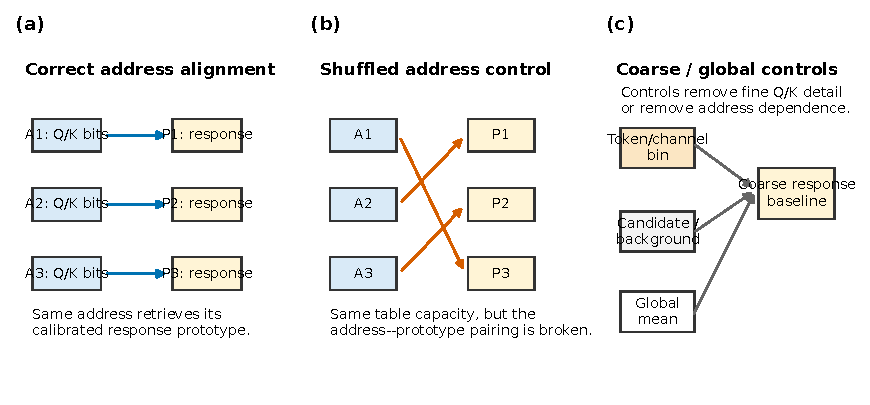
\includegraphics[width=\textwidth]{figures/fig2_address_controls.pdf}
  \caption{Negative-control protocol for address semantics. Correct-address
  lookup retrieves the response prototype calibrated for the same Q/K-derived
  address, whereas the shuffled control preserves table values and capacity but
  permutes the address--prototype mapping. Coarse token/channel,
  candidate/background, and global controls test whether reconstruction can be
  explained without fine Q/K address detail.}
  \label{fig:address-controls}
\end{figure*}

\subsection{End-to-End Current Replacement Diagnostic}
\label{sec:e2}

The replacement diagnostic substitutes the selected QKFormer attention
projection current with a hard Q/K-address lookup while the remainder of the
network executes unchanged. A static table returns the calibration-set mean
current for each supported address. The calibrated variant, referred to as
TCSLU in the experiment artifacts, applies moment and channel calibration to
restore the current distribution before the original BN/LIF path and retains
the support-aware fallback rule for missing addresses. Calibration uses 128
training batches, and classification is then evaluated on the complete
validation split with no backbone optimization.

We compare aligned addresses against shuffled address--prototype assignments,
coarse token/channel means, a global mean, and a same-size random table. We
also expand the intervention from \texttt{stage1.0.tssa} to
\texttt{stage1.0.tssa}+\texttt{stage2.0.tssa}. This evaluates classification
end to end, but the intervention remains a local current replacement rather
than replacement of every attention block or the complete QKFormer network.

\paragraph{Grouped binary-pattern projection LUT.}
The compact prototype address cannot uniquely recover every SSA projection
current. For all-attention projection replacement, we instead exploit the
binary input to each 1$\times$1 projection. Let $\mathbf{x}$ be partitioned
into $M$ groups of $g$ bits. For group $m$ and binary pattern $p$, we
precompute
\begin{equation}
  \mathcal{T}_{m}[p] = \mathbf{W}_{m}\mathbf{b}(p),
\end{equation}
where $\mathbf{W}_{m}$ contains the corresponding input columns of the frozen
projection and $\mathbf{b}(p)$ decodes the pattern. The projection current is
then reconstructed as
\begin{equation}
  \hat{\mathbf{y}} =
  \mathbf{b}_{\mathrm{proj}} +
  \sum_{m=1}^{M}\mathcal{T}_{m}[p_m(\mathbf{x})].
\end{equation}
This replaces multiplication by pattern-indexed vector lookup and
accumulation. We evaluate $g\in\{2,4,8\}$ without training. The diagnostic hook
still executes the original convolution before substituting its output, so it
tests numerical and classification fidelity rather than measured runtime.

\subsection{Downstream Validation Scope}
\label{sec:e3}

Local response reconstruction does not establish classifier improvement. We
therefore report current-replacement fidelity as a separate validation problem,
not as the basis of the compact LUT method verdict. The current study freezes
the backbone, preserves the full-validation protocol, and uses matched semantic
controls.

\paragraph{Cross-architecture protocol.}
We separately intercept the SSA projection current in Spikformer-4-384w
\cite{zhou2023spikformer}, before its original BN/LIF path, and evaluate the
same clean, static, and calibrated-current sequence on CIFAR-10 at $T=4$.
Because QKFormer and Spikformer expose different attention topology and state
geometry, this is a matched intervention protocol rather than an assertion
that their address encodings are identical. A result is considered positive
cross-architecture transfer only if the calibrated replacement is near-lossless
under fixed controls. Otherwise, the measured row is retained as an
architecture-dependent boundary. Current-level hooks do not constitute
complete model replacement.
